% mnras_template.tex 
%
% LaTeX template for creating an MNRAS paper
%
% v3.0 released 14 May 2015
% (version numbers match those of mnras.cls)
%
% Copyright (C) Royal Astronomical Society 2015
% Authors:
% Keith T. Smith (Royal Astronomical Society)

% Change log
%
% v3.0 May 2015
%    Renamed to match the new package name
%    Version number matches mnras.cls
%    A few minor tweaks to wording
%    
%    Beta testing only - never publicly released
%    First version: a simple (ish) template for creating an MNRAS paper

%%%%%%%%%%%%%%%%%%%%%%%%%%%%%%%%%%%%%%%%%%%%%%%%%%  
\documentclass[usenatbib]{mnras}
%\usepackage{newtxtext,newtxmath}
\usepackage[T1]{fontenc}


%%%%% AUTHORS - PLACE YOUR OWN PACKAGES HERE %%%%%
\usepackage{graphicx}	% Including figure files
\usepackage{amsmath}	% Advanced maths commands
\usepackage{amssymb}	% Extra maths symbols

%%%%%%%%%%%%%%%%%%%%%%%%%%%%%%%%%%%%%%%%%%%%%%%%%%

%%%%% AUTHORS - PLACE YOUR OWN COMMANDS HERE %%%%%
\newcommand{\vdag}{(v)^\dagger}
\newcommand\aastex{AAS\TeX}
\newcommand\latex{La\TeX}
\newcommand{\Msun}{\,{\rm M}$_{\odot}$\,}
\newcommand{\kms}{\,{\rm km s}\ifmmode ^{-1}\,\else $^{-1}$\,\fi}
\newcommand{\Mpch}{\,{\rm Mpc}\,\ifmmode h^{-1}\else $h^{-1}$\fi}
\newcommand{\kpch}{\,{\rm kpc}\,\ifmmode h^{-1}\else $h^{-1}$\fi}
\newcommand{\kpc}{\,{\rm kpc}\,}

%%%%%%%%%%%%%%%%%%%%%%%%%%%%%%%%%%%%%%%%%%%%%%%%%%
\title[Cosmic web elements and the $\beta$-skeleton]{Predicting the four cosmic web
  elements from the $\beta$-skeleton}


% The list of authors, and the short list which is used in the headers.
% If you need two or more lines of authors, add an extra line using \newauthor
\author[J. F. Su\'arez-P\'erez et al.]{
J. F. Su\'arez-P\'erez,$^{1}$\thanks{E-mail: jf.suarez@uniandes.edu.co}
Y. Camargo,$^{2}$ 
X.-D. Li,$^{3}$
and J. E. Forero-Romero,$^{1}$
\\
% List of institutions
$^{1}$Departamento de F\'isica, Universidad de los Andes, Cra. 1
No. 18A-10 Edificio Ip, CP 111711, Bogot\'a, Colombia\\ 
$^{2}$Departamento de F\'isica, Universidad Nacional de Colombia -
Sede Bogot\'a, Av. Cra 30 No 45-03, Bogot\'a, Colombia\\ 
$^{3}$School of Physics and Astronomy, Sun Yat-Sen University,
Guangzhou 510297, P.R.China\\ 
}

% These dates will be filled out by the publisher
\date{Accepted XXX. Received YYY; in original form ZZZ}

% Enter the current year, for the copyright statements etc.
\pubyear{2020}

% Don't change these lines
\begin{document}
\label{firstpage}
\pagerange{\pageref{firstpage}--\pageref{lastpage}}
\maketitle

% Abstract of the paper
\begin{abstract}

We show how it is possible to infer the environments of the cosmic web
of dark matter using the information of the spatial distribution
of galaxies jointly with a classic machine learning algorithm. Handled the set of galaxies as a set of nodes, we applied the
$\beta$-skeleton graph algorithm to extract geometrical information like the
number of connections or the average distance by each galaxy. 
Using these properties extracted from the distribution of galaxies was
probed the classification trees and random forest machine learning algorithms
under different configurations to find the best set of parameters that
makes a usefulness prediction with the lowest confusion.  
The results show that the average distance between galaxies on
$\beta$-graph is the most chief feature for the prediction of the
cosmic web environment.
Our methodology shows a global accuracy of $0.70$, which is an
improvement of $19$ percentual points on the total accuracy over 
other methods that predict the T-Web environment from network metrics.
Our work is a useful and simple approximation that will allow us to use
these algorithms to make predictions in observational data.
\end{abstract}

% Select between one and six entries from the list of approved keywords.
% Don't make up new ones.
\begin{keywords}
large-scale structure of Universe -- dark matter -- methods: miscellaneous
\end{keywords}

%%%%%%%%%%%%%%%%%%%%%%%%%%%%%%%%%%%%%%%%%%%%%%%%%%

%%%%%%%%%%%%%%%%% BODY OF PAPER %%%%%%%%%%%%%%%%%%
\section{Introduction}
The galaxy distribution on large spatial scales follows a structured 
pattern commonly known as the cosmic web. 
This web can be described as dense peaks connected by anisotropic
filaments and walls woven across vast under-dense voids 
\citep{Bond1996}.  
The emergence of this pattern is understood as the evolution of
initial density fluctuations growing through gravitational instability
\citep{ZelDovich1970,White1987}, a picture that can be followed in
great detail by with N-body cosmological simulations
\citep{Schmalzing1999,Vogelsberger2014}.     


There is a significant variety of methods to detect
the cosmic web in cosmological simulations.
These methods usually classify the web into four
elements: peak, filament, sheet, or void \citep{Libeskind2018}.
Most of these methods start by building a well-sampled density field
from the dark matter simulation particles.
Only a minority take as an input the discrete positions that
represent galaxies or halos.

Most of the algorithms that use discrete tracers as an input focus on
the detection of some cosmic web elements, not all of them. 
For instance, there is a great variety of void-finders
\citep{Platen2007,Neyrinck2008} and filaments-finders
\citep{Novikov2003,Zhang2009,Sousbie2010,Chen2015,Luber2019}.   
The algorithms that aim at finding the four cosmic web elements from
the galaxy positions can be roughly divided into two types.

The first type interpolates galaxy positions on a grid to process
this number density field in the same way as a dark matter density
field \citep{Eardley2015,Alpaslan2016,Tojeiro2017,Shadab2019}.
This approach has a low computational cost, but it is highly uncertain
how accurate are these results concerning the expected cosmic
web dark matter distribution.

The second type performs a full dark matter density field
reconstruction around the observed galaxies.
Most of these algorithms use Bayesian statistics coupled with Monte
Carlo sampling and N-body
simulations \citep{Jasche2010,Jasche2013a,Bos2014,LeclercqJasche2015,Horowitz2019,Burchett2020}. 
Some others are based on the density distribution around halos that
are associated to galaxy groups \citep{Wang2009,Munoz-Cuartas2011}.
This generic approach can provide accurate dark matter distributions but can
be very expensive from the computational point of view.

Recently, Machine Learning (ML) methods 
have been applied to solve the middle problem 
of finding the four web elements using dark matter halos \citep{Hui2018, Tsizh2019}.
For instance, 
\citep{Tsizh2019} classified dark matter halos 
into their cosmic web elements. 
They built networks by linking halos within a fixed linking length. 
From these graphs, 
they computed twelve different network metrics 
to feed four different ML algorithms and predict the cosmic web. The truth environments are quantified themselves over five different cosmic web classifications.

This generic procedure avoids the uncertain grid interpolation of
tracers and the expensive dark matter density reconstruction. 
Under this approach of supervised ML classification, 
the algorithm needs a feature dataset (some halo or galaxy
properties), the labels to classify the dataset (the four cosmic web
environments) and an algorithm to link the features to the classes.

The work presented here is inscribed into that line of work.
Here we show to what extent graph properties built on a galaxy
distribution can predict the cosmic web elements.
We demonstrate a specific implementation of this approach by using
the $\beta$-skeleton graph \citep{Fang2019} and the T-Web
\citep{Forero-Romero2009} classification to define the four cosmic web elements.  
We test two different supervised ML
algorithms (Classification Trees - CT, and Random Forests - RF) 
to train from the features and predict the environment.
We quantify the precision and accuracy of the algorithms using the Illustris-TNG simulation \citep{Nelson2019} at redshift $z=0$.

This paper is organized as follows. 
In Section \ref{sec:init} we describe the relevant aspects of the Illustris-TNG
simulations related to our work, the T-Web algorithm,
and the $\beta$-skeleton graph.
In Section \ref{sec:link} we describe the mechanism to link the
$\beta$-skeleton to the T-Web using machine learning algorithms.
There we detail the features and meta-parameters we use, the
classification algorithms and the metrics for model evaluation.  
In the Section \ref{sec:results} we present our results. In the Section \ref{sec:discussion} we explore a brief discussion comparing our results with other methods 
to finally summarize our conclusions in Section
\ref{sec:conclusions}.

\section{Initial Algorithms and Simulations}\label{sec:init}

\subsection{Illustris-TNG}

The
Illustris-TNG project \citep{Nelson2019} is a series of large,
cosmological gravo-magnetohydrodynamical and semi-analytical simulations of galaxy formation. 
These simulations are based on the cosmological standard model
$\Lambda$CDM and uses the \texttt{AREPO} code \citep{Springel2011}.
The simulations run start from the cosmology $\Lambda$CDM with the
cosmological parameters: cosmological constant
$\Omega_{\Lambda,0}$=0.6911, matter density $\Omega_{m,0}$=0.3089,
baryonic density $\Omega_{b,0}$=0.0486, normalization
$\sigma_8$=0.8159, spectral index $n_s$=0.9667 and Hubble constant
$H_o$= 100$h\,km\,s^{-1}\,Mpc^{-1}$ with $h$=0.6774 consistent with
the Planck 2015 results \citep{Ade2016}.  

The Illustris-TNG project simulates different structures in the visible matter like stars, black holes, or diffuse gas jointly with the distribution of dark matter.
The project includes simulated galaxies as realistic as possible to
make a comparison with the real universe. There are 18 different
simulations with boxes of sizes $50$ Mpc, $100$ Mpc, and $300$ Mpc that started at $z=127$ and finalized at $z=0$.    

In this work we used the TNG300-1\footnote{TNG300 has 3 different resolutions, 1 is refer to the highest resolution.}  (~300 Mpc) simulation at $z=0$.
This simulation has a volume of 302.6$^3 cMpc^3$, with a baryonic mass resolution of 88$\times 10^{6}$ \Msun  and dark matter mass resolution of 470$\times  10^{6}$ \Msun \citep{Nelson2019}.
The number of galaxies in TNG300-1 at $z=0$ is 14M 
with a total of 711M stars simulated. 
The simulation includes sub-grid stellar and black hole evolution process together with its associated 
feedback processes \citep{Nelson2019,Pillepich2018a,Springel2018}.

In the TNG300-1 simulation, the galaxies are called subhalos and are defined as any gravitationally
bound object with a nonzero
stellar component.
To identify galaxies in the simulation,
first, a friends-of-friends group finder is run
in order to identify FOF haloes with
a linking length $l=$ 0.2,
within which gravitationally bound substructures
are then located and classified hierarchically \citep{Pillepich2018a}.
 
\subsection{T-Web Classification}

\begin{figure}
\centering
 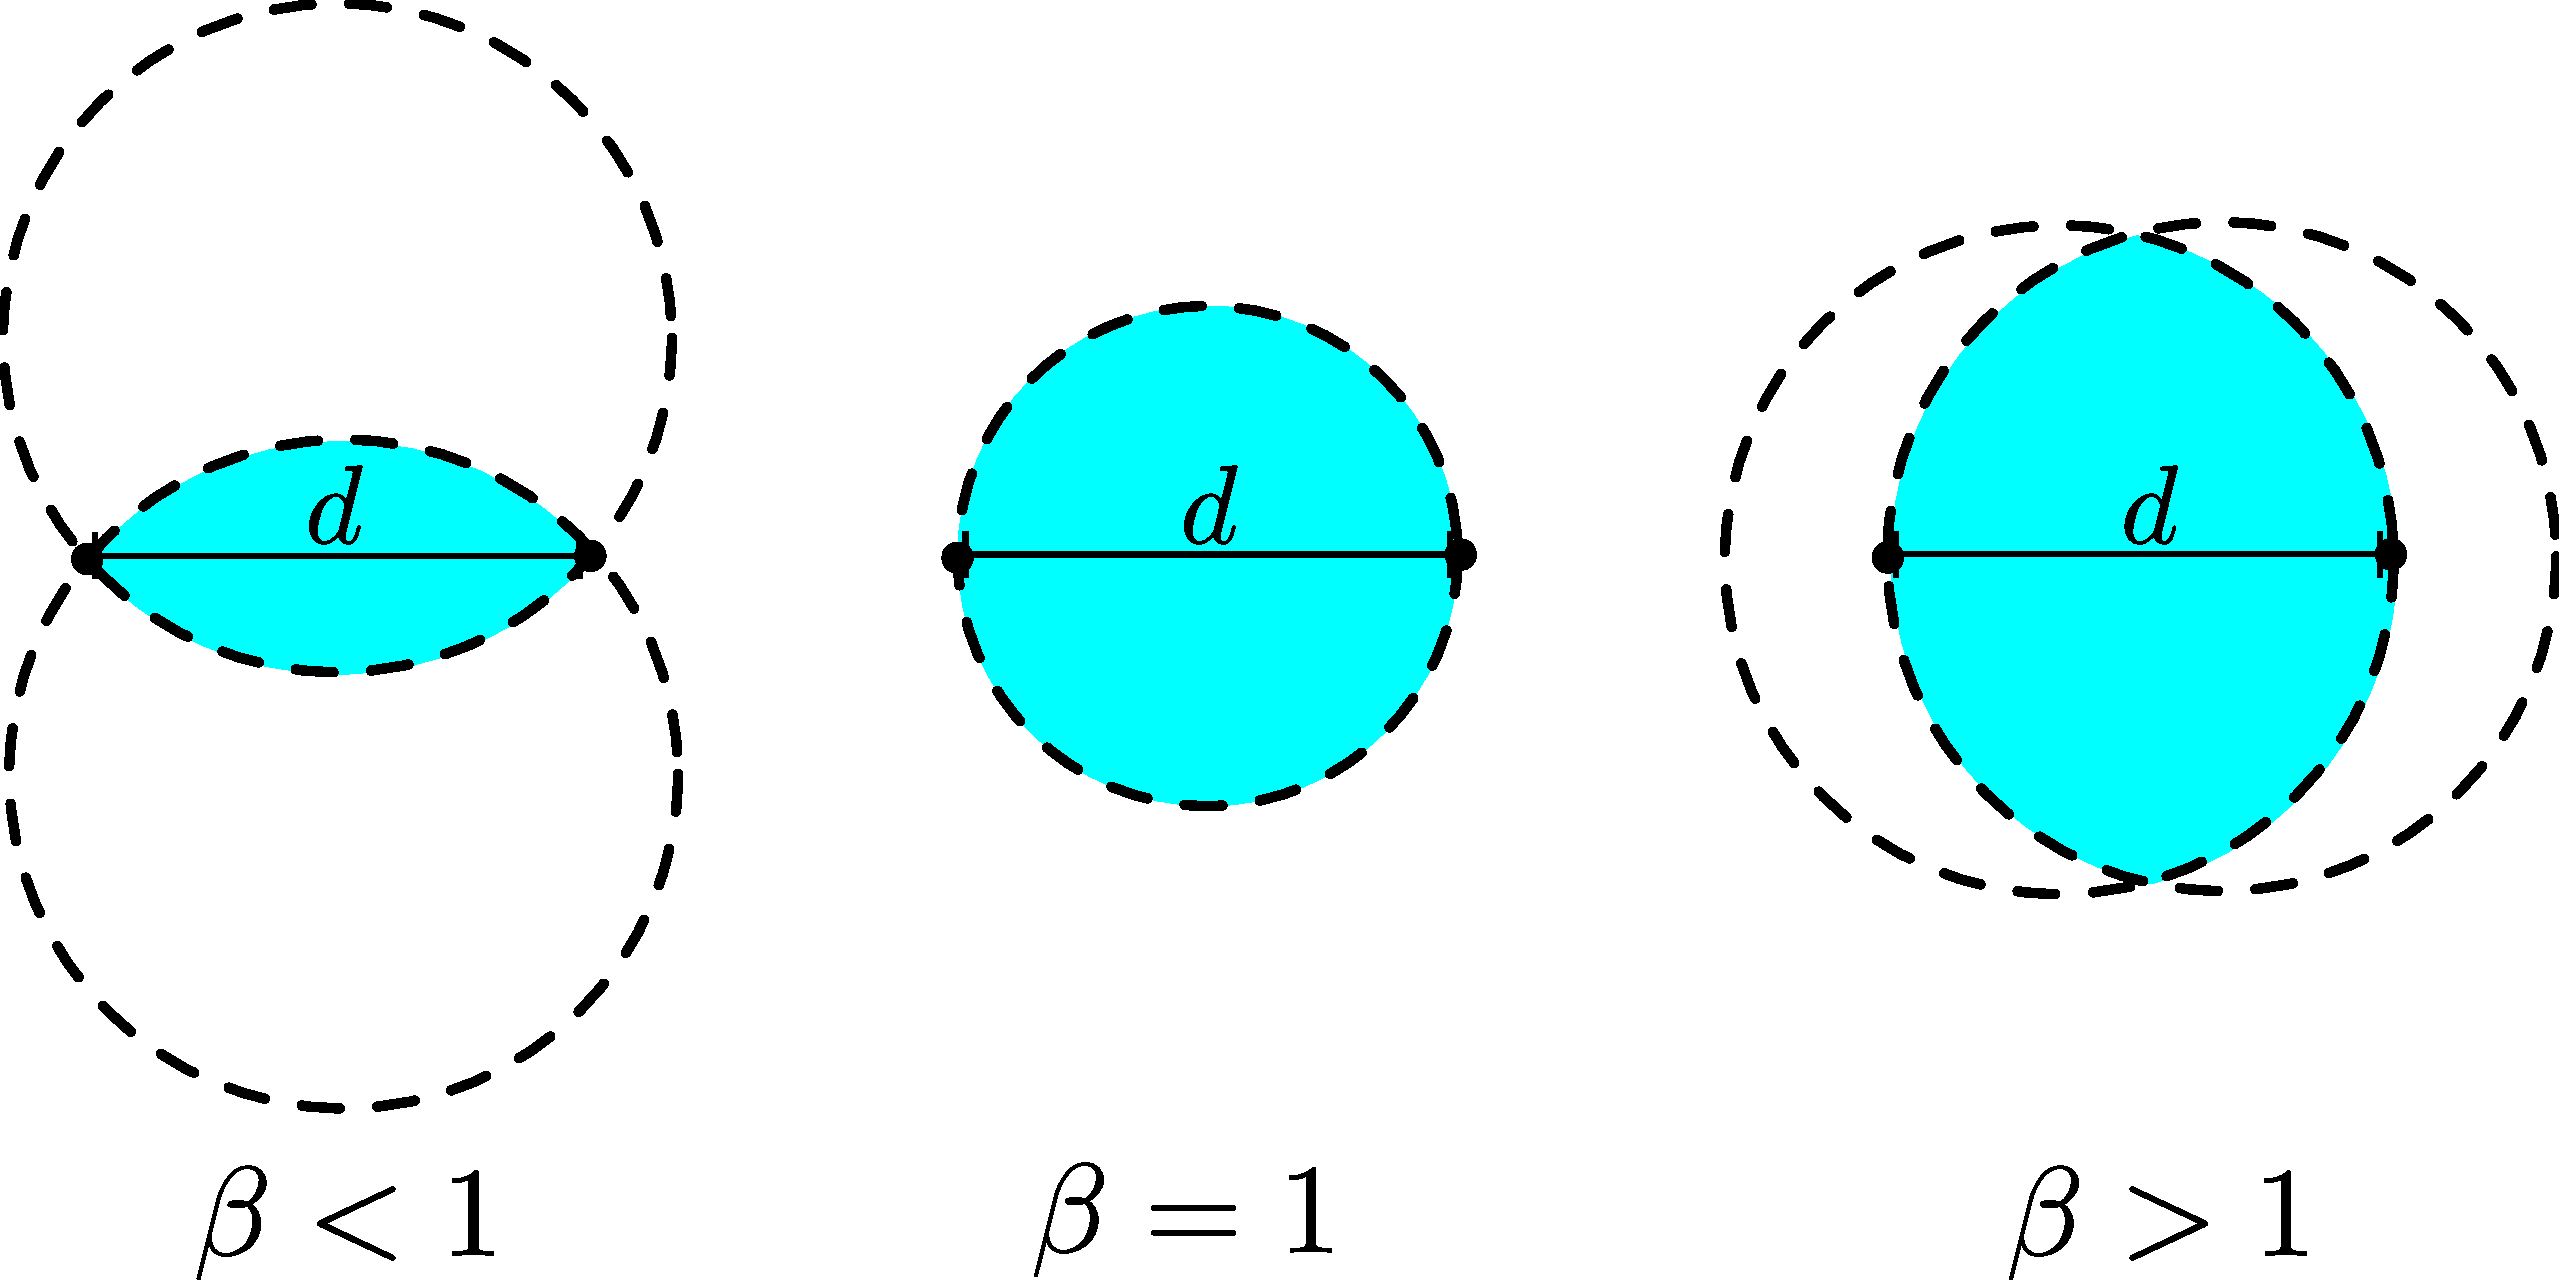
\includegraphics[scale=0.18]{Figs/p_beta.pdf}
 \caption{Exclusion region of the $\beta$-skeleton under the Lune-based definition.}  
 \label{fig:beta}
\end{figure}

The tidal web (T-Web) method \citep{Hahn2007, Forero-Romero2009}
classifies the large scale structure into four web types: voids,
sheets, filaments, and peaks.   
This classification is based on the eigenvalues of the deformation
tensor $T_{\alpha\beta}$, the Hessian of the gravitational potential 
\begin{equation}
T_{\alpha\beta}=\frac{\partial^2\psi}{\partial r_{\alpha}r_{\beta}},
\end{equation}
%
where $\psi$ is a normalized gravitational potential that follows the equation
\begin{equation}
    \nabla^2 \psi = \delta,
\end{equation}
%
and $\delta$ is the dark matter overdensity.
This tensor has three real-valued eigenvalues. 
The cosmic web environment is defined by the number of eigenvalues
larger than a threshold value $\lambda_{th}$.
Locations with three eigenvalues larger than $\lambda_{th}$ correspond
to a peak, two to a filament, one to a sheet, and zero to a void.


 
\begin{figure*}
\centering
 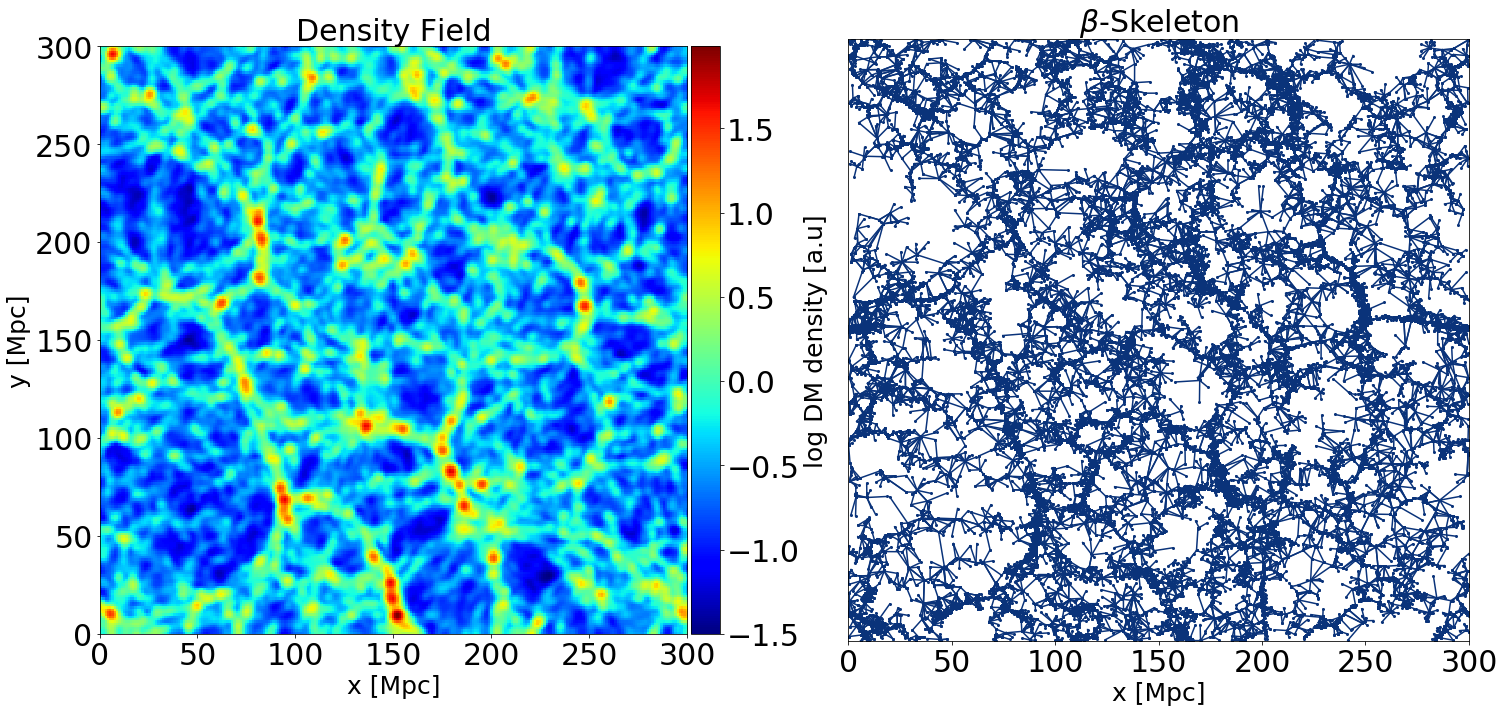
\includegraphics[scale=0.3]{Figs/p_Fig1_.png}%Figs/p_TWeb_bsk.pdf}
 \caption{Comparison between the T-Web of dark matter density field
   (left) and the $\beta$-skeleton (right) computed from the
   distribution of galaxies with $\beta$=1 for TNG300-1.}  
 \label{fig:TWebBsk}
\end{figure*}


Computationally speaking, to define an environment in an N-body
simulation we implement the following seven steps: 1) interpolate the
mass particles with a Cloud-In-Cell (CIC) scheme over a grid to
obtain the density, 2) smooth it with an isotropic Gaussian filter,
3) compute the overdensity, 4) find the normalized potential with Fast
Fourier Transform  methods, 5) compute the deformation tensor using
finite differences, 6) find the eigenvalues, and finally 7) count the
number of eigenvalues larger than the threshold $\lambda_{th}$.  


\begin{figure*}
        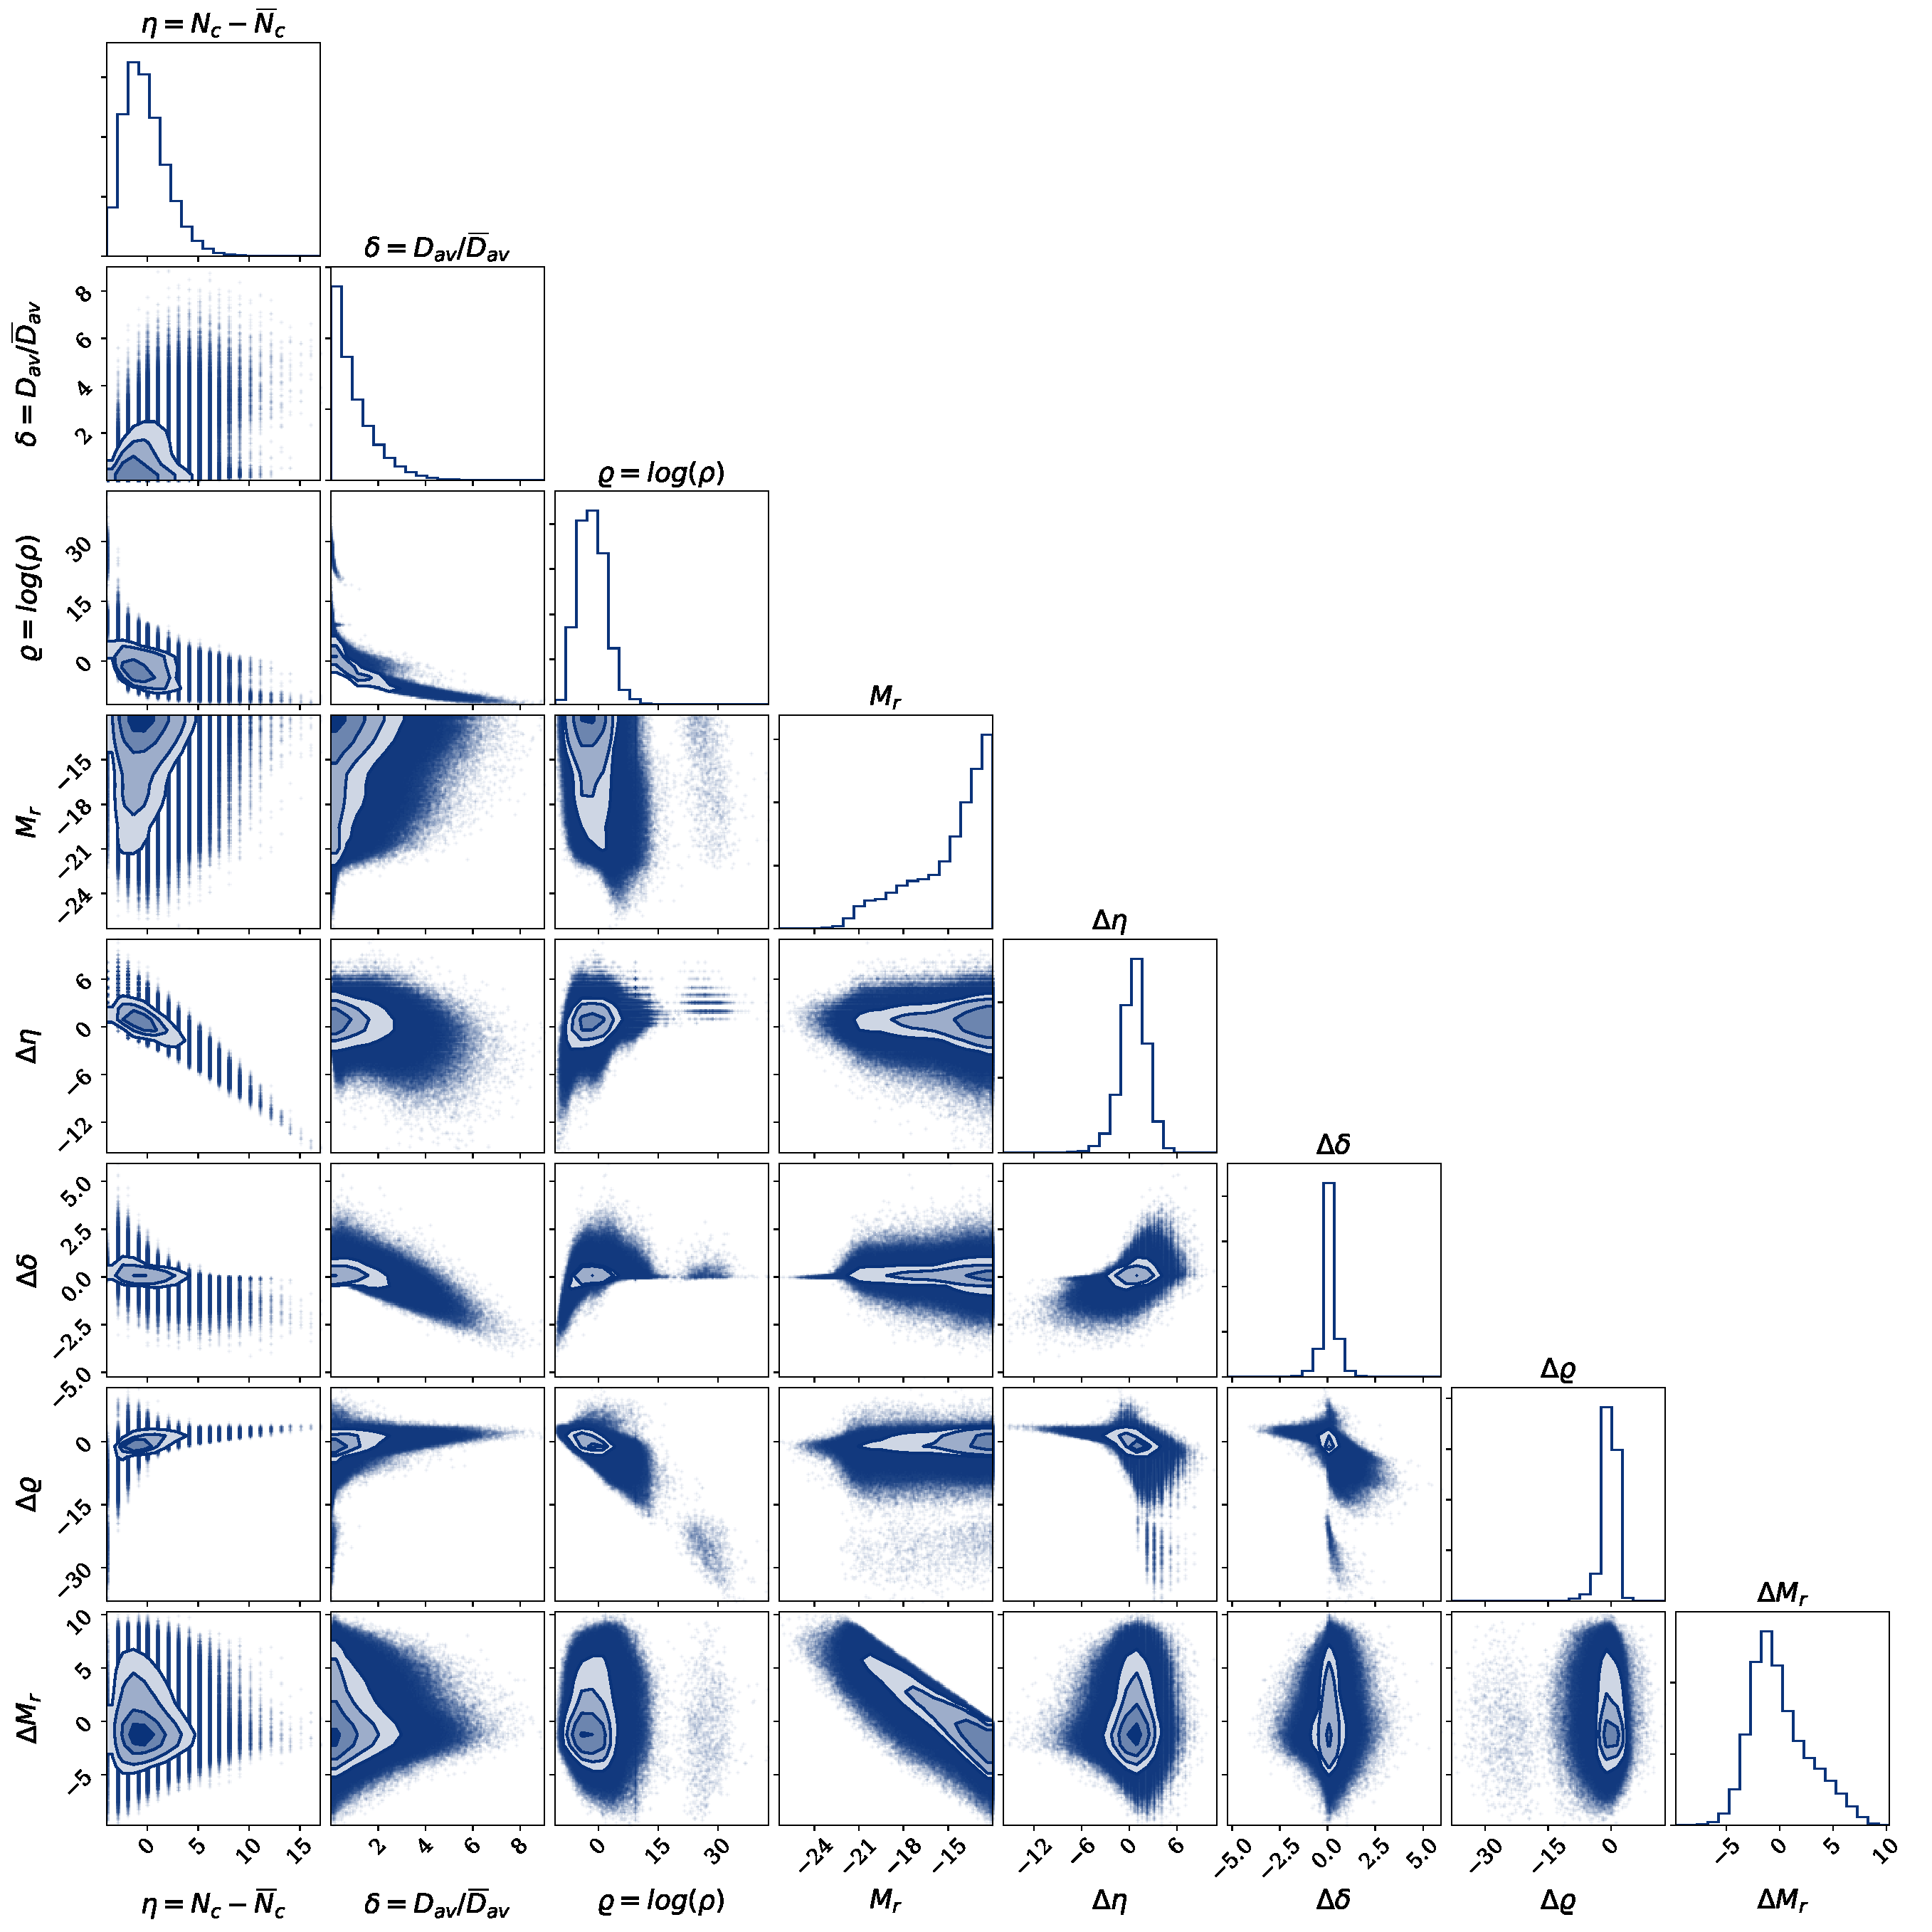
\includegraphics[scale=0.46]{Figs/p_all_features_correlations.pdf}
    \caption{Histograms and correlations curves for the six features
      used to train the classifiers. These features were extracted from the 1-skeleton graph.}
    \label{fig:features}
\end{figure*}

\subsection{The $\beta$-skeleton algorithm}


The $\beta$-skeleton is an algorithm that computes a graph over a
distribution of nodes \citep{Kirkpatrick1985, Fang2019}.  
This algorithm depends on a positive and continuous parameter $\beta$
that defines an exclusion region between two nodes.

Defining $d$ as the distance between two nodes, they are connected by
an edge if any other point is allocated in the various exclusion
regions shown in Figure \ref{fig:beta}.  

For $\beta<1$, the exclusion region is the intersection of all the 
spheres with diameter $d/\beta$ that pass through the nodes. In the
case, $\beta=1$, the exclusion region is a sphere with a diameter $d$.
As $\beta$ increases, $\beta>1$, the exclusion region is larger and it
is the intersection of all the spheres with diameter $d\beta$ having
the nodes in their boundary.  

This makes that for low values of $\beta$ the graph is dense and for
large values of $\beta$ the graph become sparse. 
The $1$-skeleton also receives the name of Gabriel Graph.  
The $2$-skeleton is also known as the Relative Neighbor Graph (RNG).

In our case, the galaxies represent a node in the graph.
From this graph, we compute a variety of features to be used as an input for the classification task.

\section{Linking the $\beta$-skeleton to the T-Web}\label{sec:link}

Figure \ref{fig:TWebBsk} shows the correlation between the dark matter overdensity
and the $\beta$-skeleton graph computed over the corresponding galaxy
distribution. 
This spatial correlation suggests that graph derived features might have
a good chance to predict the dark matter web environment. 
However, there is a number of free parameters that have to be explored
to find the best match between the $\beta$-skeleton and the cosmic web.

\subsection{T-Web and $\beta$-skeleton free parameters}

For a start, the influence of the $\beta$ parameter has to be explored.
Additionally, the classification provided by the T-Web algorithm
depends on the smoothing scale, $\sigma$, used to compute the Hessian and the
threshold parameter $\lambda_{th}$ used to define the web elements.
The tracers we use from the simulation can also change. 
We use a simple magnitude cut $M_{r}$ on the $r$-band absolute magnitudes
to define the galaxy sample. 
Different values for that threshold naturally produce different galaxy
distributions and thus different $\beta$-skeletons. 

The T-Web computation is performed over a cubic grid with $256^3$
cells. 
This corresponds to a cell size of $1.17$Mpc.
For the smoothing parameter, we take five different values of $\sigma =
0.5$, $1.0$, $1.5$, $2.0$ and $2.5$, expressed in units of the cell size on a side.
In turn, for each smoothing length we take six different values for
the eigenvalue threshold
$\lambda_{th}=0.0, 0.1, 0.2, 0.3, 0.4$ and $0.5$. 
We use four different values for the limiting $r$-band magnitude
$M_{r}$, we use  $-18, -16, -14$ and $-12$.
From these galaxies, we compute the skeleton using values of $\beta$ in
the range $1\leq \beta \leq 2$ to find that the best results are
obtained for $\beta=1$.
Therefore we keep this value fixed for the results reported here.

Once these four different parameters ($\beta$,
$\sigma$, $\lambda_{th}$ and $M_{r}$) are fixed the $\beta$-skeleton and the
T-Web are fixed.  
Next, we define what features used to predict the four cosmic web elements.

\subsection{Galaxy Features}
We use six features for each galaxy in the $\beta$-skeleton to train the classifiers. 

\begin{enumerate}
\item[1)]
The number of connections minus the global median number of
connections, $\eta = N_c - \bar{N}_c$. 
\item[2)]
The ratio between the average edge length to first neighbors on the graph
normalized by the global average edge length, $\delta=D_{av}/\bar{D}_{av}$. 
\item[3)] 
The logarithm of the pseudo-density over the graph,
  $\varrho=\log_{10}\rho$.   
This pseudo density $\rho$ is defined as the inverse of the volume
computed from the ellipsoid that best fits the distribution of first
neighbors over the graph. 
If a galaxy has less than three neighbors its volume is fixed to be $10^{-4}$.
\end{enumerate}
\noindent
We define three more features that we call $\Delta$-features.
Their values are computed as the difference between the corresponding
value in a node and the average value over first neighbor nodes.  
They can be loosely interpreted as a first derivative computed over the graph. 

\begin{enumerate}
\item[4)] $\Delta$ over the number of connections, $\Delta\eta$.
\item[5)] $\Delta$ over the normalized edge length, $\Delta\delta$.
\item[6)] $\Delta$ over the the pseudo-density, $\Delta\varrho$.
\end{enumerate}

Figure \ref{fig:features} shows the correlations among all features.
The diagonal panels present the distribution of a given parameter.
The strongest correlations are present for the average number of
connections $\eta$, the connection length $\delta$ and the
pseudo-density $\varrho$ with their
corresponding $\Delta$ features.


\subsection{Classification Algorithms}

We explore two different supervised machine learning algorithms to
predict the cosmic web environment from the features we have just presented.
For each algorithm, the most relevant meta parameters driving their
performance.

\begin{itemize}
    \item Classification Trees (CT):
      \begin{itemize}
      \item Maximum tree depth: From 1 to 30.
      \end{itemize}
    \item Random Forest (RF):
        \begin{itemize}
            \item Maximum tree depth: 10.
            \item Number of estimators: From 1 to 100.
        \end{itemize}
\end{itemize}

\subsection{Model evaluation}

After computing the features, we divided the full simulated box into eight boxes with the same volume, 150$^3$ $Mpc^3$. Then, we discard the galaxies located within 5 Mpc away from the boxes limits to avoid boundary effects coming from incomplete $\beta$-skeleton information.  
From this dataset, we selected the galaxies allocated in four boxes that represent a $50\%$ of the full volume, this selection is used to train the ML algorithms.
We use other two boxes, i.e. a $25\%$ volume, as validation to find the best algorithm and ML
meta-parameters together with the best matching T-Web and
$\beta$-skeleton parameters.   
Finally, we use one other box, a $12.5\%$ of volume, as test to report
on the expected confusion matrix and feature importance for the classification. The remaining box was published in the repository of the project on \href{https://github.com/jsuarez314/cosmicweb_bsk}{github}. It is a mock example to evaluate the best model.

As performance metrics, we compute the precision, recall and the F1
score (harmonic mean between precision and recall).  
We compute the F1 for each web environment and its average.


\begin{figure}
    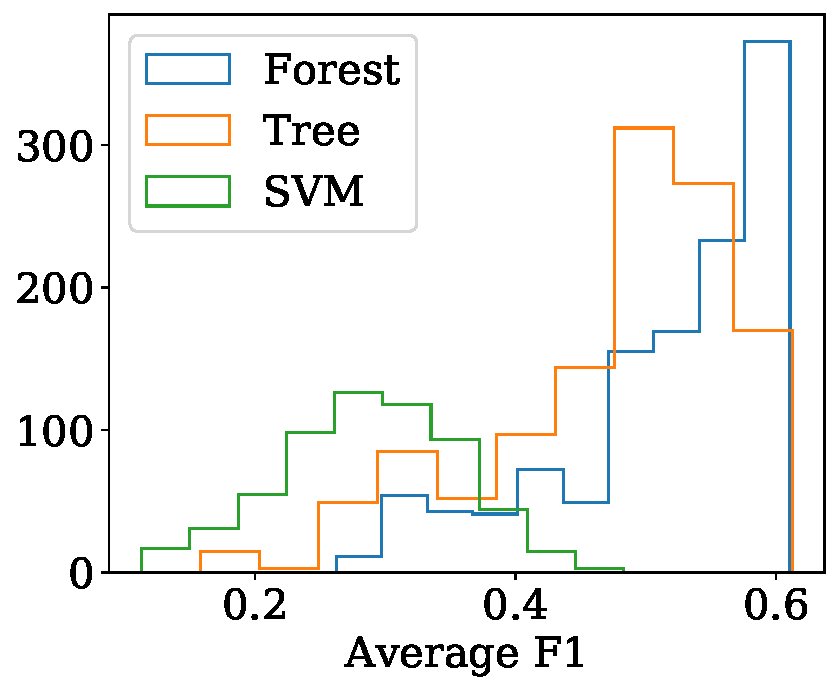
\includegraphics[scale=0.55]{Figs/p_hist_f1.pdf}
    \caption{Histograms of the average F1 for the two machine
      learning algorithms, Random Forest (RF) and Classification Trees (CT).
      The average F1 changes as the parameter and meta-parameter are changed.}
    \label{fig:methods}
\end{figure}


\begin{figure*}
\centering
    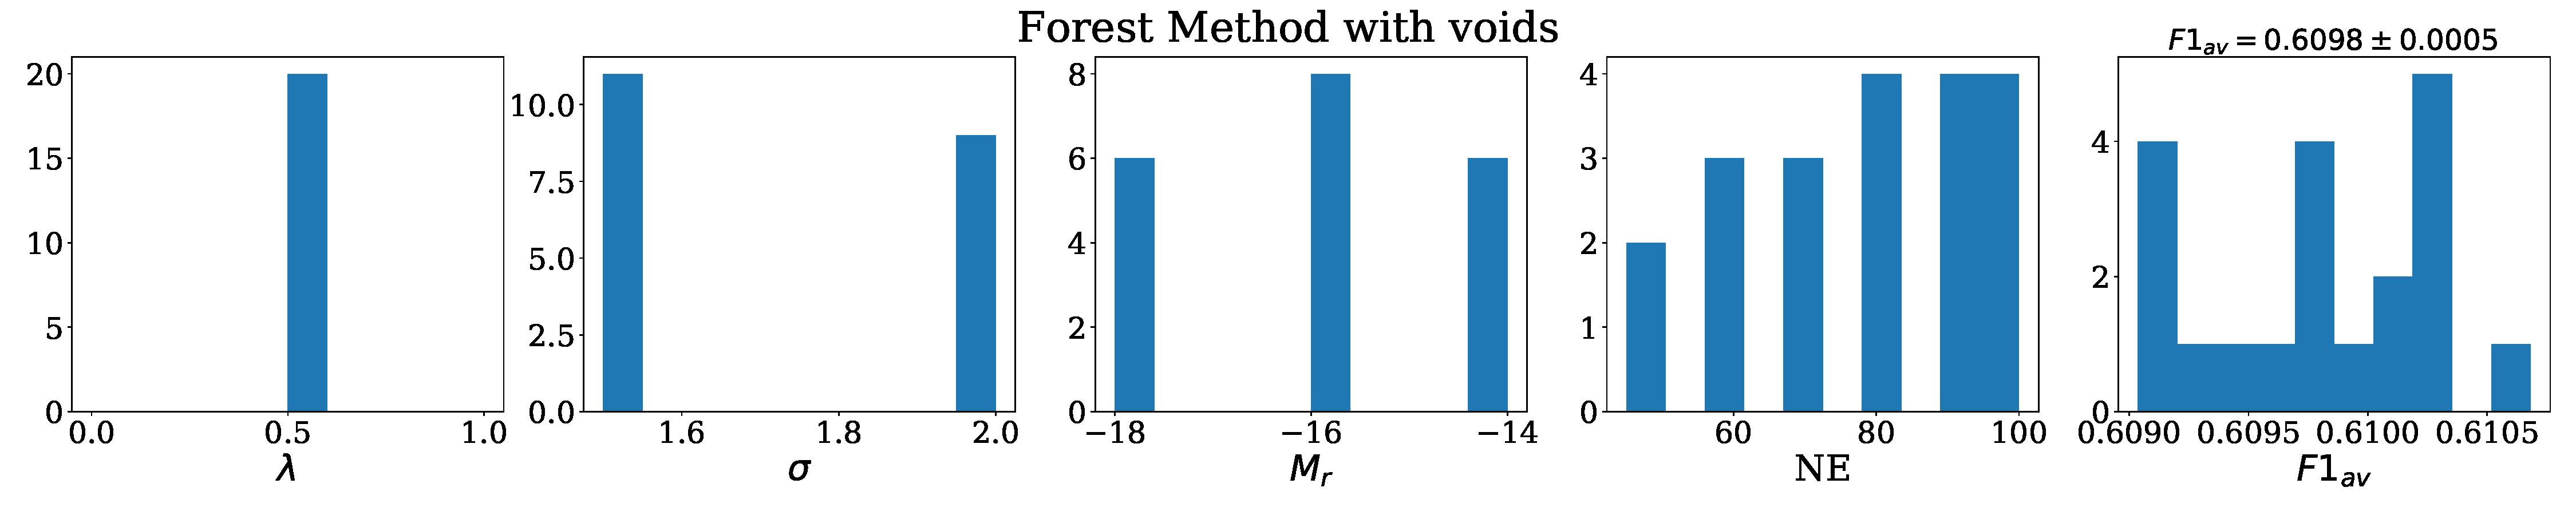
\includegraphics[scale=0.23]{Figs/p_features_Forest_F1_av.pdf}
    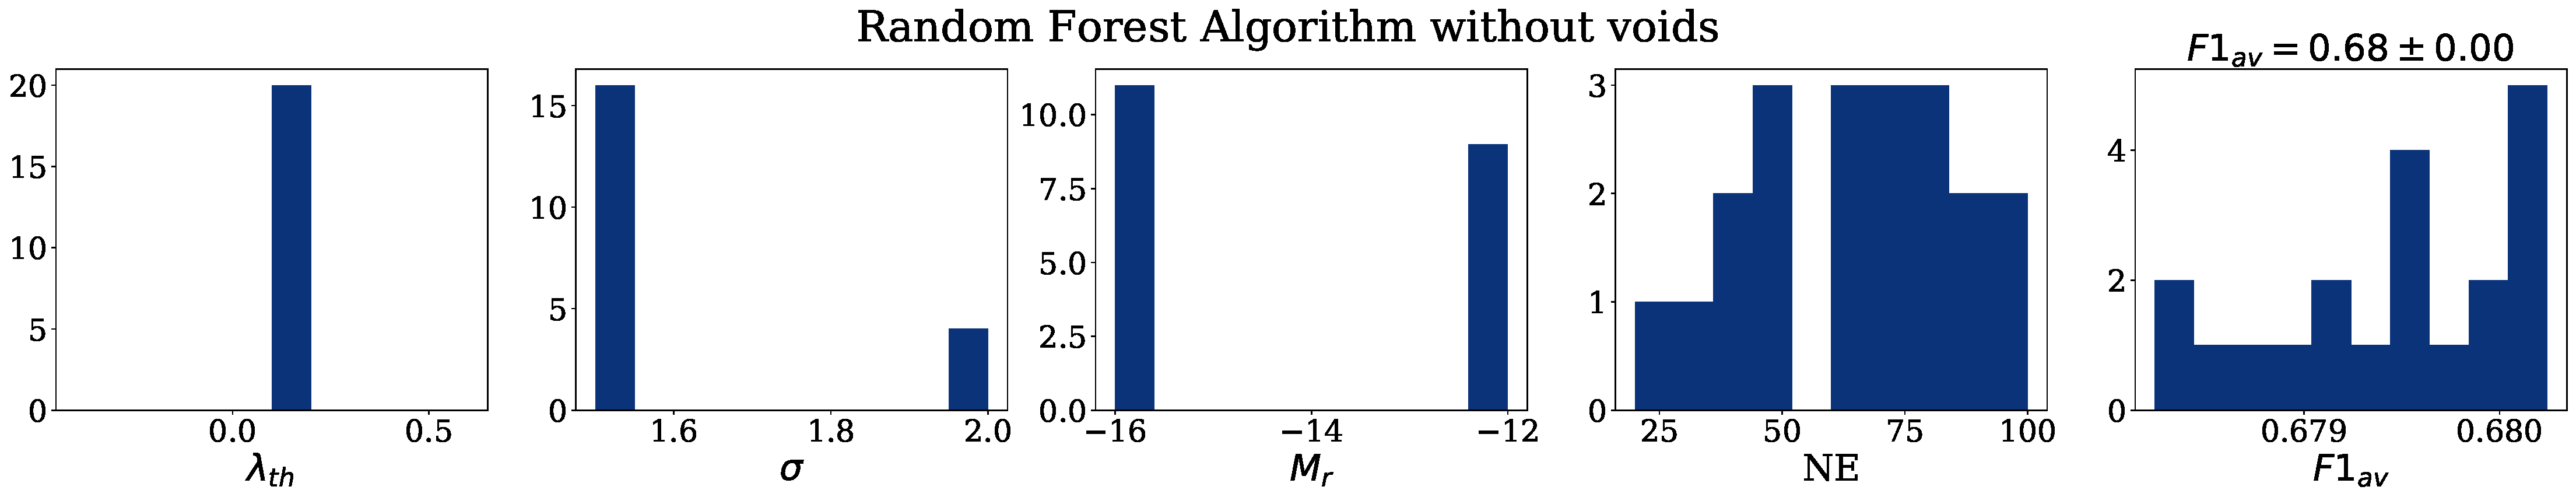
\includegraphics[scale=0.23]{Figs/p_features_Forest_F1_av_no_voids.pdf}
    \caption{(Upper) Distribution of the meta-parameters and the F1 average for the best 15 models when the voids are including in the average. We can observe that  the $\lambda_{th}$ meta-parameter is 0.5, $\sigma$ is 1.5, $M_r$ jumps from -14 to -16, and the $NE$ is concentrates around 80.
    (Bottom) Distributions when the voids are not including in the average. We can observe that the $\lambda_{th}$ meta-parameter is 0.1 and 0.2, while $\sigma$ is 1.5, $M_r$ is -14 and also the $NE$ is concentrates around 80.
      } 
    \label{fig:features_score}    
\end{figure*}


\begin{table}
\centering
\begin{tabular}{ccc}
\hline
 F1-score                   & RF              & TC              \\
\hline
 $F1_{\rm peaks}$               & 0.54 $\pm$ 0.27 & 0.52 $\pm$ 0.18 \\
 $F1_{\rm filaments}$           & 0.72 $\pm$ 0.05 & 0.64 $\pm$ 0.07 \\
 $F1_{\rm sheets}$              & 0.56 $\pm$ 0.07 & 0.50 $\pm$ 0.06  \\
 $F1_{\rm voids}$               & 0.29 $\pm$ 0.18 & 0.28 $\pm$ 0.14 \\
 $F1_{\rm avg}$ including voids    & 0.53 $\pm$ 0.09 & 0.49 $\pm$ 0.07 \\
 $F1_{\rm avg}$ excluding voids & 0.61 $\pm$ 0.09 & 0.55 $\pm$ 0.07 \\
\hline
\end{tabular}
\caption{Mean values and standard deviations over the F1
  scores for all models in each one of the ML algorithms.
  The first four rows differentiate the results for each one of the
  environments.
  The fifth row corresponds to the unweighted average over the four
  web elements, while the last row is the average over web elements
  with the exclusion of voids.}
\label{table:elements}
\end{table}


\section{Results}\label{sec:results}

\subsection{ML algorithm performance}


We start by comparing the performance of the different ML algorithms.
Figure \ref{fig:methods} shows the average F1 distribution for
all the classification experiments.
The histograms are discriminated into the two ML algorithms.
From these two models, the results from the Random Forest (RF) are
better; the F1 value distribution is skewed towards higher values than
the distribution from the Classification Trees.
From this overall response over all possible models, Random Forest
emerges as the best ML algorithm.
We can confirm this result by performing a more detailed analysis by
taking a look at the results for each cosmic web element separately.

Table \ref{table:elements} summarizes the F1 performance split by cosmic
web element in the first four rows.
The mean values and standard deviations are computed over all the ML experiments. 
From this table, we confirm that the Random Forest (RF) classifier performs
consistently better than Classification Trees (CT) for every web element.
The F1 scores comparison between RF and CT shows that for filaments and
sheets the RF produces average F1 scores 0.07 higher. 
However, for peaks and voids the average of the scores is similar. 

\subsection{Performance across web elements}

Table \ref{table:elements} also shows that some cosmic web elements 
are harder to predict than others.
Focusing our attention on the RF classifier, the algorithm with the
best results, we readily observe that filaments is the environment
with the best mean F1 score (0.72).
This score is followed by sheets and peaks (0.56 and 0.54,
respectively) and finally by voids (0.29).

Void is the hardest class to predict. 
The reason behind this result is easy to understand. 
There are too few galaxies in voids.
Across all models, less than $0.4\%$ of all galaxies
are classified as void galaxies.
This has two consequences.
First, the low number of instances makes it hard for the ML algorithm to
define the region in parameter space occupied by voids.
Second, a small number of void galaxies that are misclassified is translated into large changes in the F1 scores.

In comparison, Filament is the class with the best score.
For RF classifier, the F1 score for filament is the highest of all four
web elements with an average value of  $0.72$.
Notably, the F1 dispersion across models is also the lowest
corresponding to $0.05$.
Galaxies in filaments are also the most represented,
approximately $58.6\%$ of all galaxies are classified as filament galaxies.
This helps to explain that it is easier for the ML algorithm to learn
the characteristics that make a galaxy sit in a filament.
Sheet and Peak have intermediate F1 scores between
those for Void and Filament, with average values of $0.56$ and $0.54$.
The fraction of galaxies in Sheets and Peaks averages are $19.8\%$ and $21.3\%$, respectively. 

The failure to classify voids has to be taken into account at the
moment of assigning a global score to a model.
Not taking into account these special results can be misleading.
The reason for that is we have used the average F1 across the
four classes to define that algorithm was better. 
We should also compute the average F1 across classes, but
\emph{excluding voids}.
This is what we do in the last two rows in Table \ref{table:elements}.
In what follows we keep in mind this distinction in order to provide a
fairer evaluation for each model.


\subsection{Best match between T-Web and $\beta$-skeleton}

We now focus on understanding what are the best matched T-Web and
$\beta$-skeleton parameters.
In this exploration, we focus on the algorithm that we already know
provides the best classification results: Random Forest. 
To do that we choose the best $N=15$ models in terms of their average F1 across
classes and see what do they have in common.
Choosing $N=10$ or $N=20$ does not have a great impact on our
results. 
However, as we previously saw, including voids or not in the analysis
has deeper consequences that we are going to explore next.

Figure \ref{fig:features_score} summarizes the parameter and meta-parameter
distribution for the best $N=15$ models in the Random Forest
classification.
The upper raw takes voids into account for the F1 average computation,
while the lower raw does not.
The panels in each row have the following meaning.
The first two panels show the T-Web parameters
$\lambda_{th}$ and $\sigma$, the third panel corresponds to the $M_r$
absolute magnitude cut that impacts the $\beta$-skeleton, the fourth panel is the meta-parameter Number of estimators ($NE$) in the RF
classifier and finally the last panel shows the average F1 across classes for the best N models. 

Excluding the void F1-score or not has a dramatic influence on
on the preferred valued for $\lambda_{th}$. 
If the void F1-score is included in the average F1 the preferred value is
$\lambda_{th}=0.5$. 
This preferred value drops to $\lambda_{th}=0.1$  if voids are not taken into account in the average score.
Why is this difference relevant?
Pushing $\lambda_{th}$ towards high values makes the voids larger.
That means that more galaxies are included in voids, giving the ML algorithm more instances to train, explaining the rise in the F1 score for $\lambda_{th}=0.5$.

However, the T-Web voids corresponding to $\lambda_{th}=0.5$ are unphysical: they have densities a few times above the mean
density and are so large that they occupy $60\%$ of the total volume.
In other words, the $\lambda_{th}=0.5$ voids are actually including regions that would be classified as sheets
\citep{Bustamante2015, Forero-Romero2009}. 

For those reasons we decide to exclude the F1-score for voids in
judging what model is best.
This choice is equivalent to computing the average F1-score using the
four environments, but weighted by the number of instances. 
The weighted average score automatically gives less importance to the
less represented class, which in this case corresponds to voids.

\begin{table}
\centering
\begin{tabular}{cccc}
\hline
   $\lambda$ &   $\sigma$ &   $M_r$ &   $NE$ \\
\hline
         0.1 &        1.5 &     -14 &     20 \\
         0.2 &        1.5 &     -14 &     40 \\
         0.2 &        1.5 &     -14 &     50 \\
         0.2 &        1.5 &     -14 &    100 \\
         0.1 &        1.5 &     -14 &     30 \\
         0.2 &        1.5 &     -14 &     90 \\
         0.1 &        1.5 &     -14 &     80 \\
         0.1 &        1.5 &     -14 &    100 \\
         0.1 &        1.5 &     -14 &     40 \\
         0.2 &        1.5 &     -14 &     70 \\
         0.1 &        1.5 &     -14 &     90 \\
         0.1 &        1.5 &     -14 &     70 \\
         0.2 &        1.5 &     -14 &     60 \\
         0.1 &        1.5 &     -14 &     60 \\
         0.2 &        1.5 &     -14 &     80 \\
\hline
\end{tabular}
\caption{Values of the meta-parameters for the best 15 models using Random Forest with the validation data when we do not include the voids in the F1 average score.}
\label{tab:parameters}
\end{table}

All the other parameters ($\sigma$, $M_r$ and $NE$) give similar results.
The best value for $\sigma$ is 1.5, the preferred values
for $M_r$ is $-14$ and the best Number of
Estimators $NE$ is around $80$.
To decide on the best set of parameters we use the results listed in
Table \ref{tab:parameters}.
There we list the 15 parameter combinations that
produce the highest F1 weighted average values.
From that list we find that the combination that appears more often is 
\{$\lambda_{th}=0.1$, $\sigma=1.5$, $M_r=-14$\} followed by 
\{$\lambda_{th}=0.2$, $\sigma=1.5$, $M_r=-14$\}.
For the Number of Estimators, we pick $NE=80$.



\subsection{Confusion Matrix and Feature Importance}

We finalize this section by reporting the results from the model 
\{$\lambda_{th}=0.1$, $\sigma=1.5$, $M_r=-14$, $NE=80$\}.
These results are computed on the reserved $12.5\%$ test data that has not be used so far.

Figure \ref{fig:confusion_matrix} shows the confusion matrix.
The numbers correspond to the fraction of objects that correspond to
the \verb"Truth" class but are classified into the \verb"Prediction"
class.
What are the most common misclassifications?
In first place comes the $86\%$ of void galaxies that are misclassified
as sheet galaxies.  
In second place we have the $44\%$ of sheets that are misclassified
as filaments, and finally, the $34\%$ of peaks that are misclassified as filaments.

\begin{figure}
\centering
    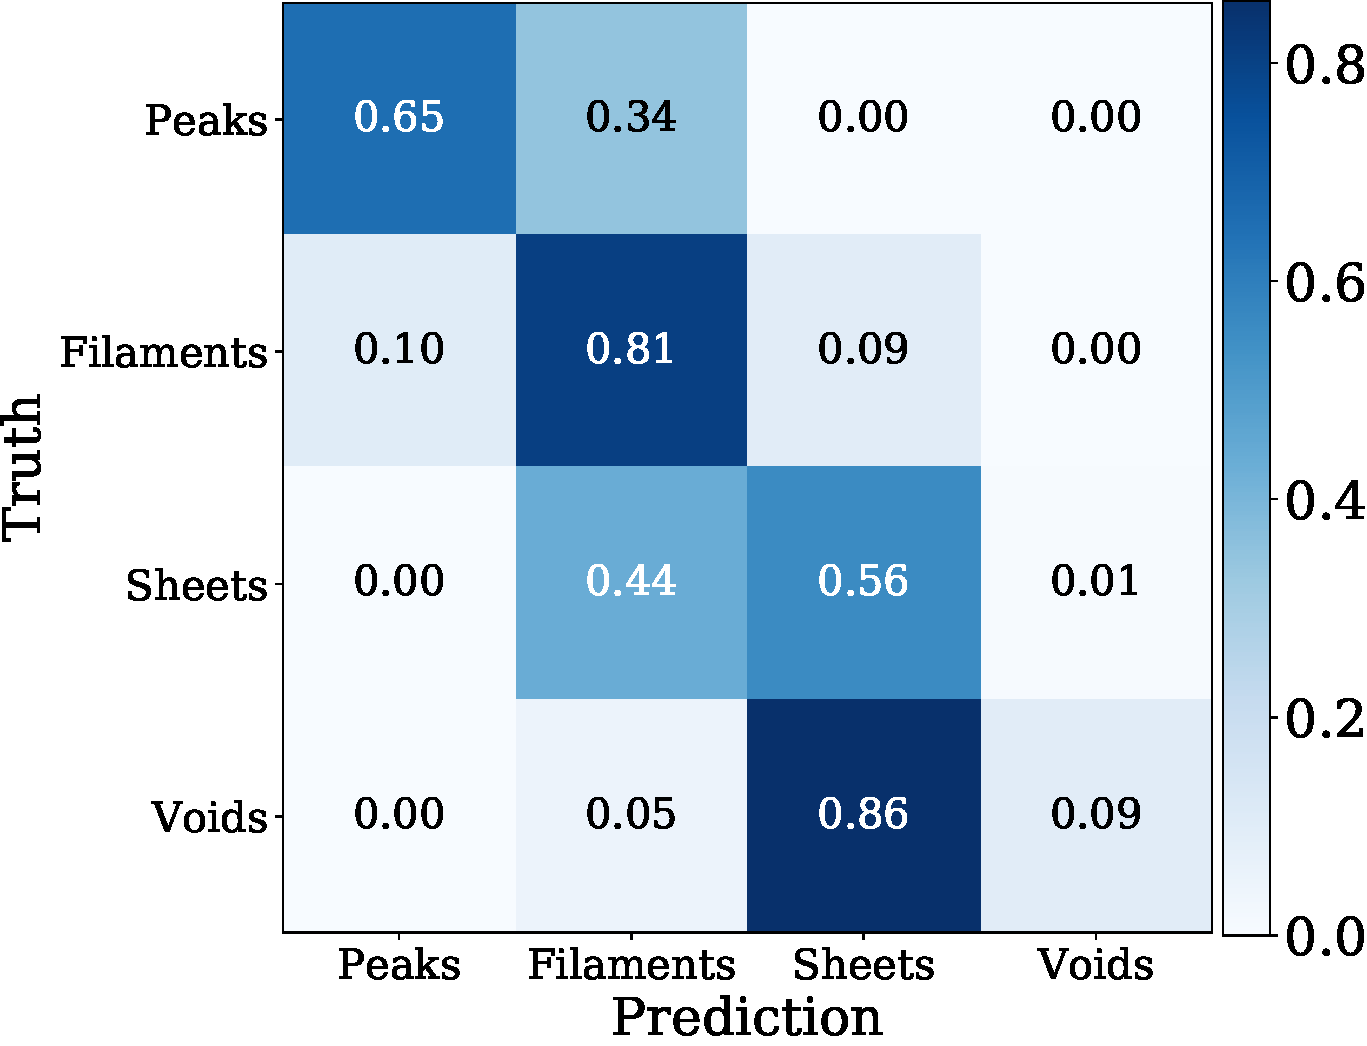
\includegraphics[scale=0.35]{Figs/p_confusion_matrix_test.pdf}
\caption{Confusion matrix for the model 
      \{$\lambda_{th}=0.1$, $\sigma=1.5$, $M_r=-14$,
      $NE$=80\} computed on the test dataset.}
      \label{fig:confusion_matrix}
\end{figure}

\begin{figure}
    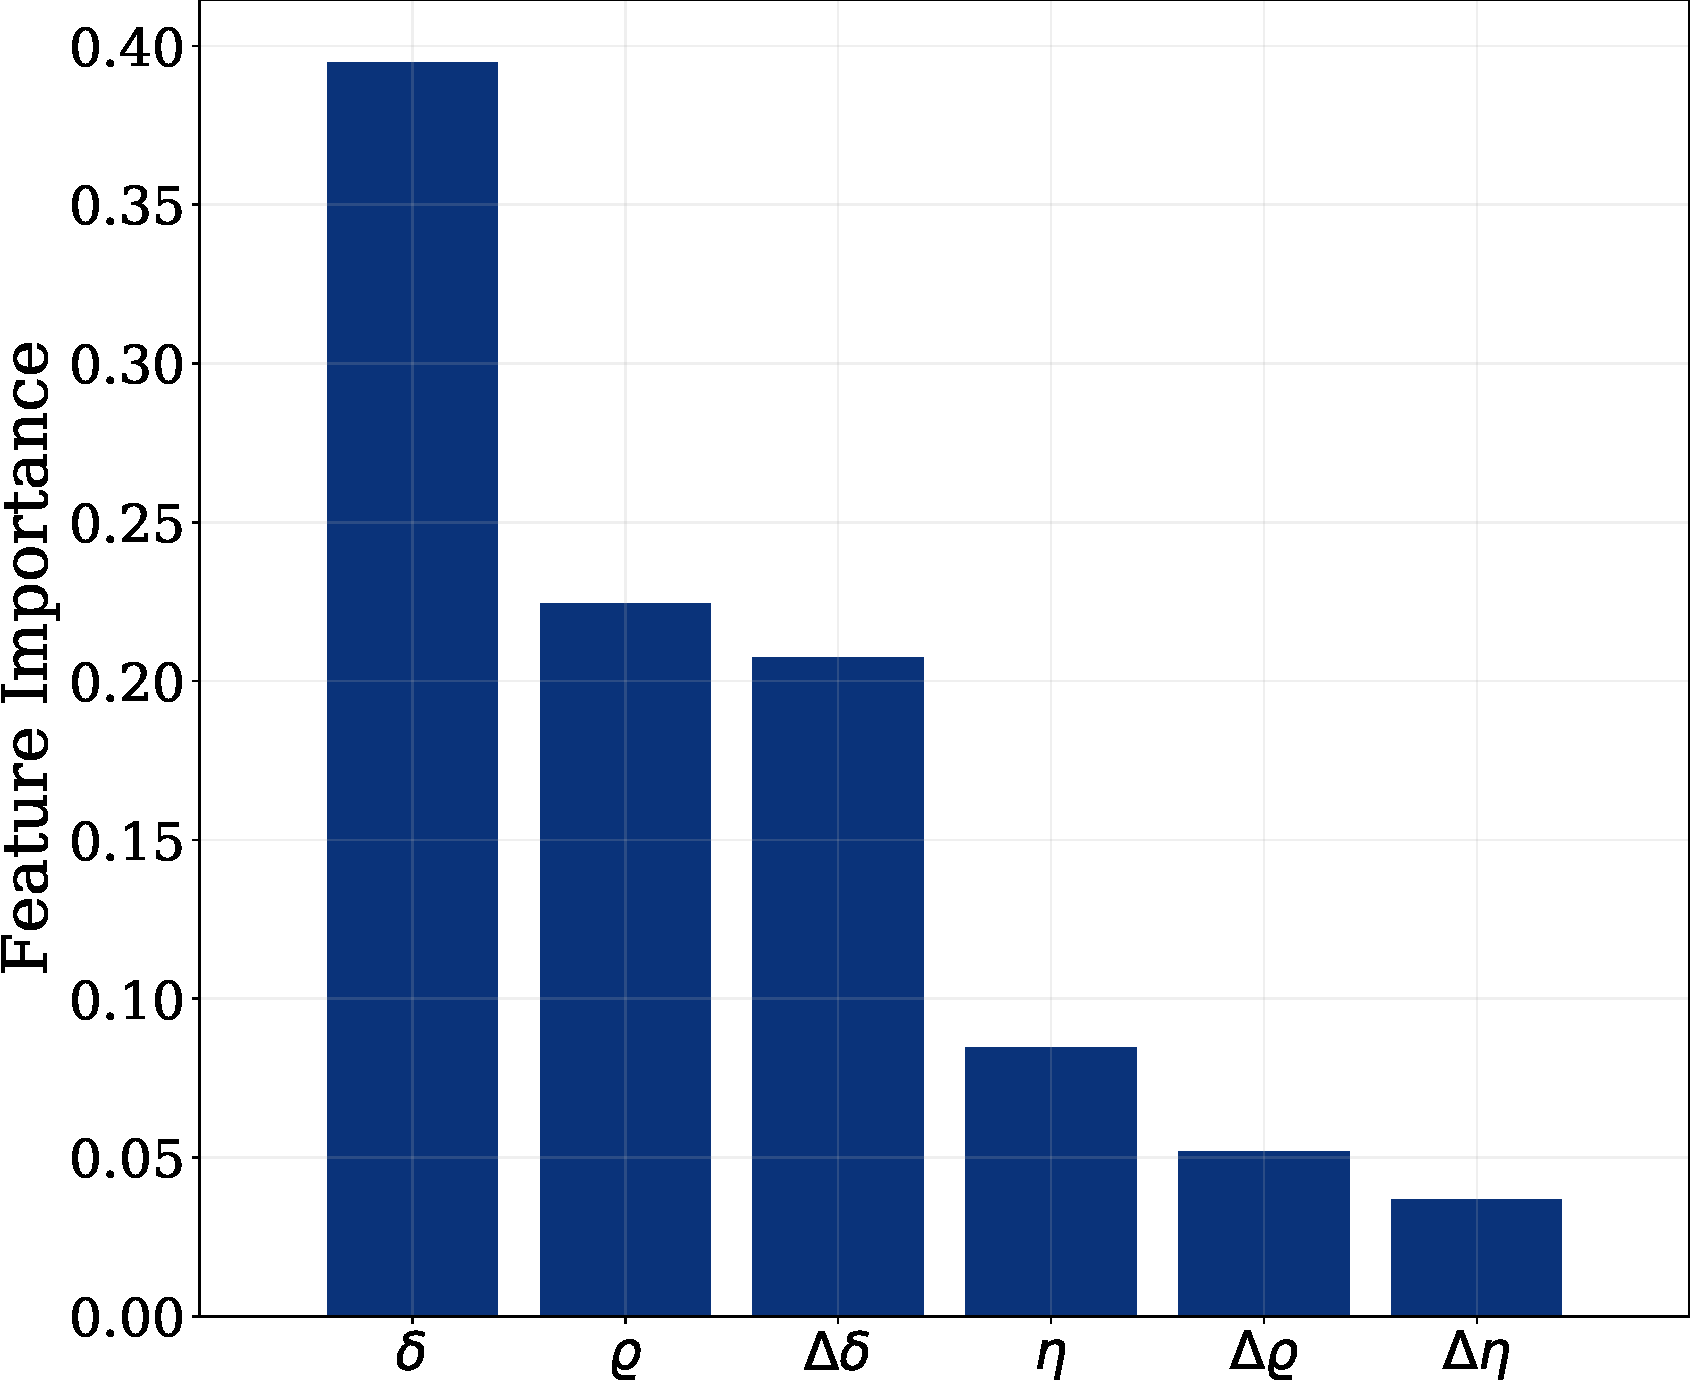
\includegraphics[scale=0.29]{Figs/p_features_importance_test.pdf}  
    \caption{
      Feature importance in the Random Forest classifier for the model
      \{$\lambda_{th}=0.1$, $\sigma=1.5$, $M_r=-14$,
      $NE$=80\} computed on the test dataset.}
    \label{fig:feature_importance}
\end{figure}

\begin{figure*}
  \centering 
    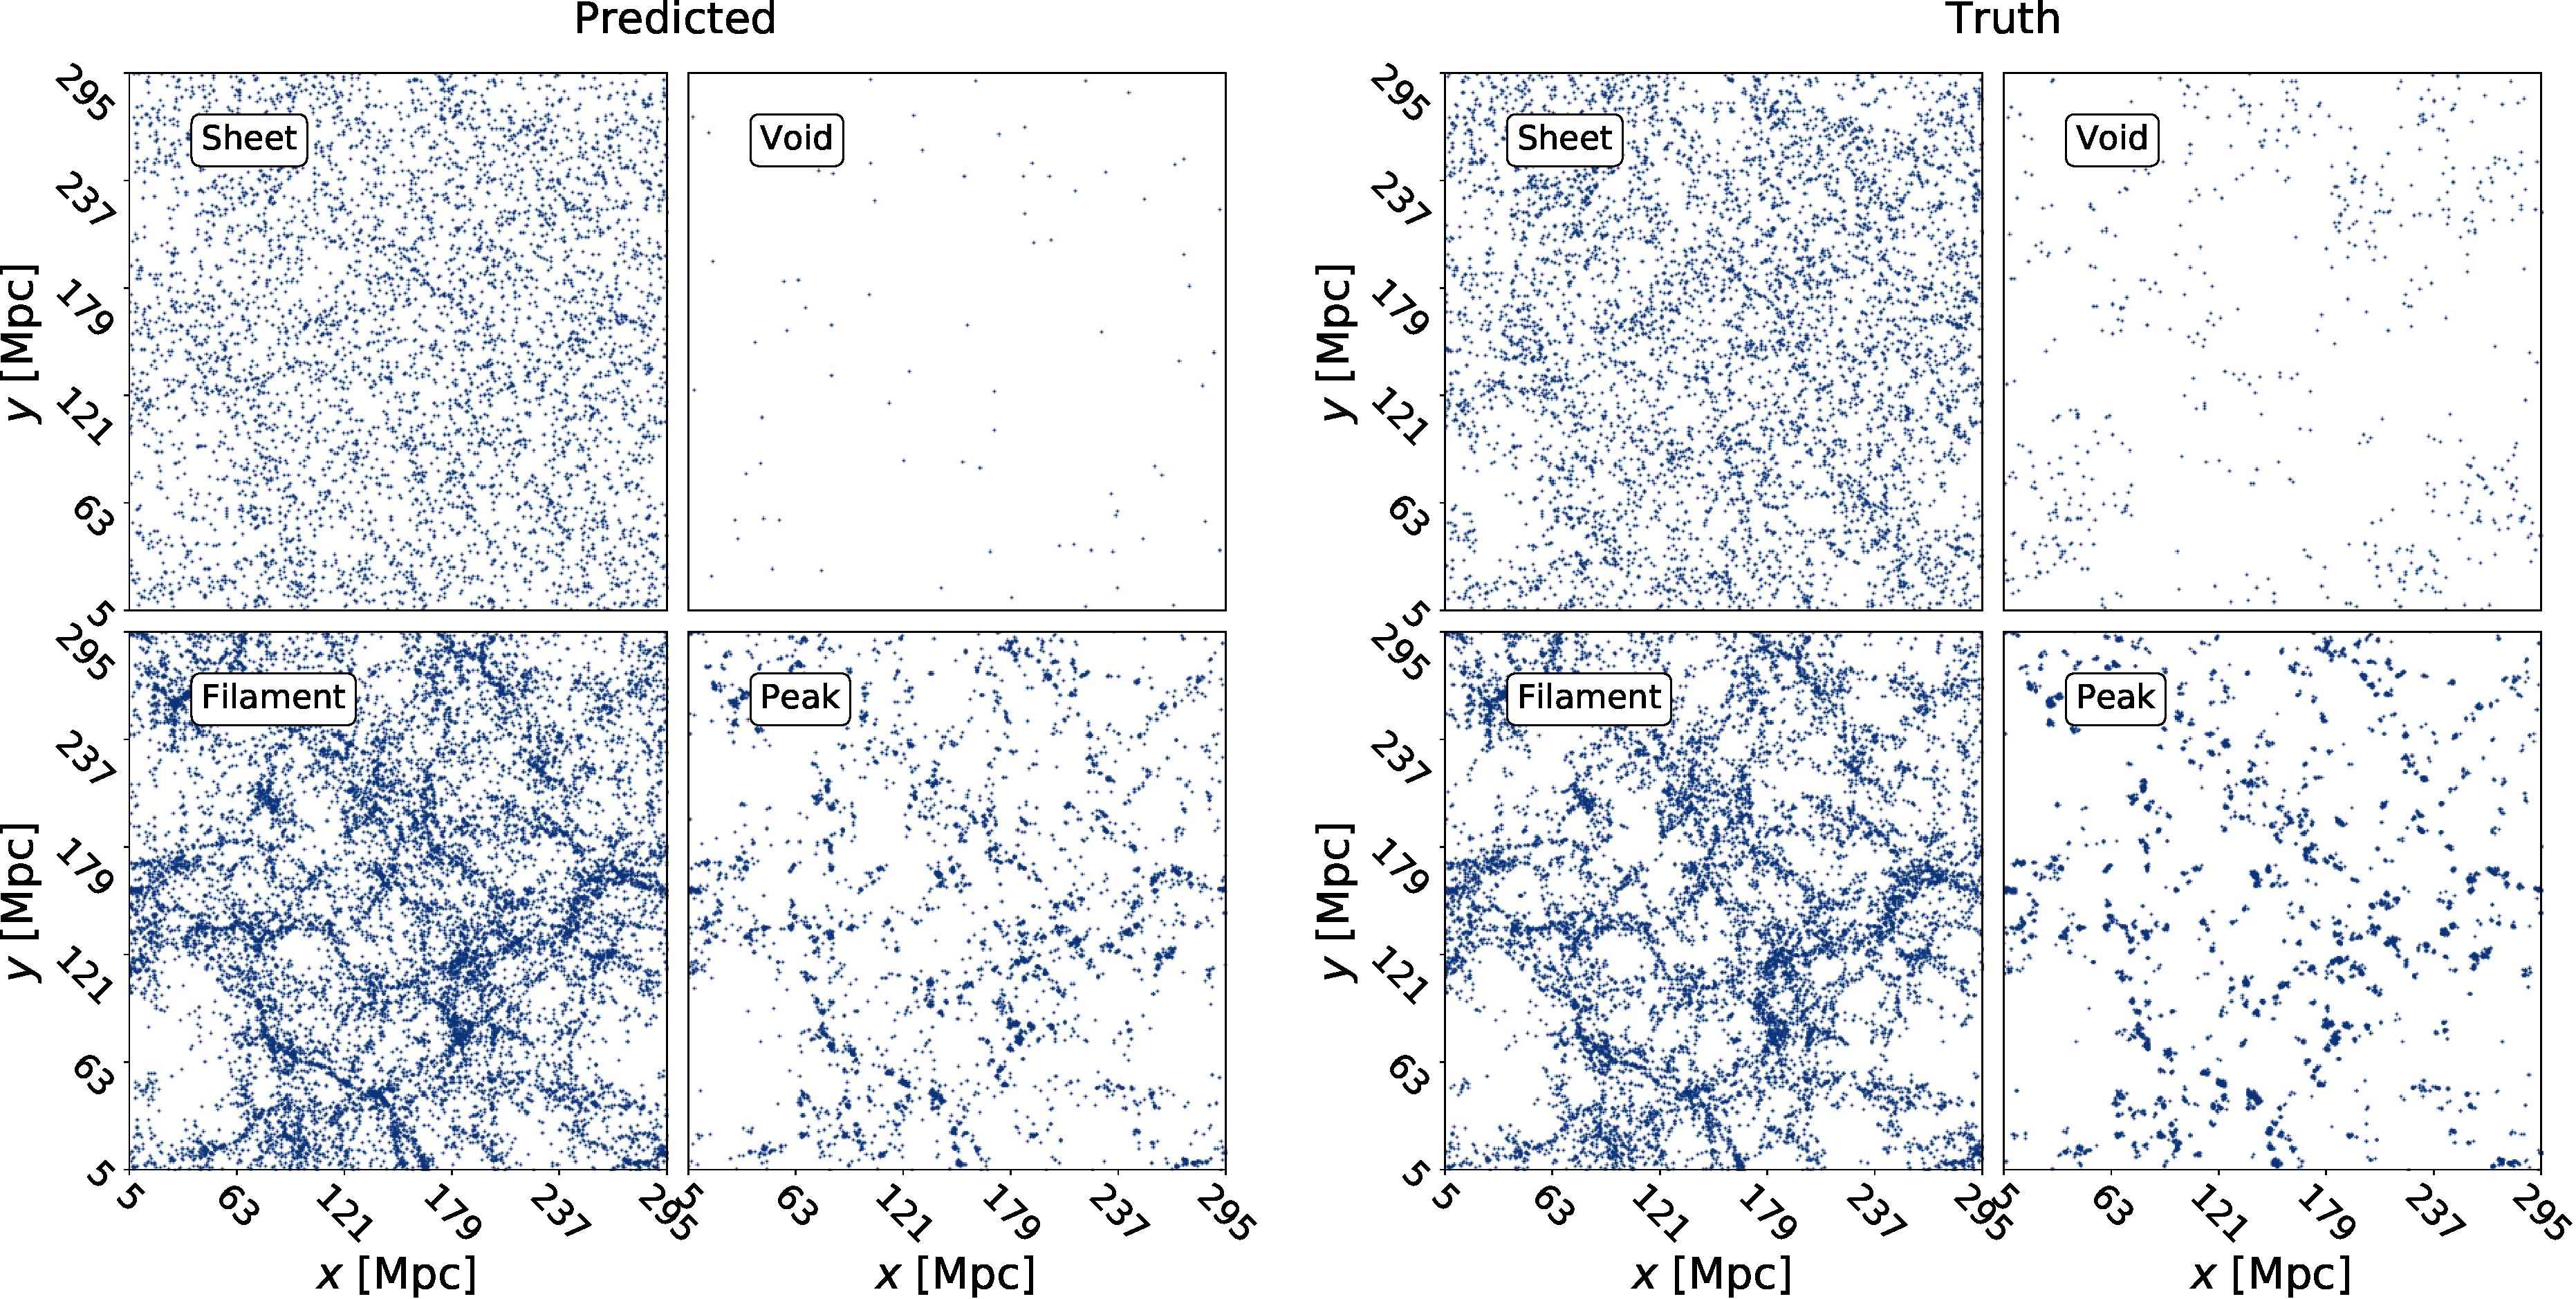
\includegraphics[scale=0.28]{Figs/p_environment_predicted.pdf}
    \caption{Spatial distribution for the galaxies classified into the
      four web elements following the T-Web environment (left) and 
      the $\beta$-skeleton based prediction (right).} 
    \label{fig:prediction}
\end{figure*}

The first misclassification results highlight the difficulty to find void galaxies.
This turns out to be an almost impossible task for one simple reason:
there are very few void galaxies.
The second kind of misclassification shows that the galaxies
classified as belonging to a filament, actually belong to neighboring
environments: sheets and peaks.

This misclassification can also be understood in terms of the
topological properties of the cosmic web elements. 
Voids are surrounded by sheets, sheets have filaments inside them and
filaments in turn have peaks inside them \citep{Cautun2014}. 
In this progression the average density increases and the tidal field
anisotropy goes from being isotropic (voids) to anisotropic (sheets
and filaments) and isotropic (peaks) \citep{Bustamante2015}.

The ranking of correct classifications follows the F1 trends
shown in Table \ref{table:elements}.
Filaments are the class most correctly classified ($80\%$) followed by
peaks ($70\%$) and sheets ($60\%$).
Void galaxies have the worst results, only $10\%$ of void galaxies are
correctly classified.
This ranking follows the trend in the fraction of instances belonging to
filaments ($51\%$), peaks($25\%$), sheets ($22\%$), and voids ($2\%$).
A higher number of instances translates into a better chance for the
algorithm to give a correct classification. 

Figure \ref{fig:feature_importance} shows the feature
importance for the classification.
In the combination of six features the four most important ones are:
$\delta$ (average edge
length), $\varrho$ (pseudo density), $\Delta \delta$ (changes in the average edge length), $\eta$ (number of connections) 
The most interesting outcome is that the average length and the pseudo-density turn out to be crucial for the classification.

Figure \ref{fig:prediction} summarizes our results.
It shows the spatial distribution for the galaxies into the four web
elements. 
The left panel correspond to the prediction from the
$\beta$-skeleton features and the right panel to the T-Web
computation.
The failure in the void classification is visible as an excess of
galaxies classified as belonging to a void, compared to the lower
number in the T-Web classification.
A similar trend, although less pronounced is visible for peak
galaxies, although the predictions seem to have a similar clustering
as the input truth. 
On the other hand, sheet galaxies in the prediction appear more
dispersed than they should.
Finally, the visual impression for filament galaxies is the most
similar between truth and prediction, as expected by the quantitative
results presented here.


\section{Discussion}\label{sec:discussion}

\begin{table}
\centering
\begin{tabular}{c|c|c|c|c|}
\cline{2-5} &
\multicolumn{2}{c|}{\textbf{\begin{tabular}[c]{@{}c@{}}Best
      Model\\ Tsizh et al. (2020) \end{tabular}}} &
\multicolumn{2}{c|}{\textbf{\begin{tabular}[c]{@{}c@{}}Best Model\\ 
This Work \end{tabular}}} \\ \hline
\multicolumn{1}{|c|}{\textbf{Class}}     & \textbf{Score}   &
\textbf{Tracer \%}   & \textbf{Score}     & \textbf{Tracer \%}  \\ \hline
\multicolumn{1}{|c|}{\textbf{Peaks}}     & 0.41   & 5.0\%   & 0.65  & 25.4\%   \\ \hline
\multicolumn{1}{|c|}{\textbf{Filaments}} & 0.62   & 19.9\%  & 0.81  & 50.5\%   \\ \hline
\multicolumn{1}{|c|}{\textbf{Sheets}}    & 0.64   & 38.8\%  & 0.56  & 22.3\%   \\ \hline
\multicolumn{1}{|c|}{\textbf{Voids}}     & 0.82   & 36.4\%  & 0.09  & 1.9\%    \\ \hline
\end{tabular}
\caption{Comparison of the diagonal elements of the confusion matrix
  (Scores) between the best models in \citep{Tsizh2019} and our work.
  Comparing each class in the two classifications we see that a higher
  score correspond to a higher tracer percentage.}
\label{tab:tsizh}
\end{table}

A similar methodology proposed in \citep{Tsizh2019} combines a complex
network analysis with ML to predict the environments in the cosmic
web. In that paper, the nodes are represented by dark matter halos in
a box with length of 290 Mpc extracted from the \texttt{GADGET-2}
cosmological simulation \citep{Springel2005}. The halos in the
simulation were identified by a friends-of-friends algorithm to create
a catalog \citep{Libeskind2018}. The catalog has a total of 281465
halos with mass range from 10$^{11}h^{-1}$ to
10$^{15}h^{-1}$\Msun. Over the distribution of halos was computed 10
network metrics by node. To compute these metrics was created a graph
from the position of the nodes and a linking length
$l=$2$Mpch/h^{-1}$. The metrics together with the mass and the
peculiar velocity make up the input data for the ML algorithms. In
comparison with our work, we use the positions of 392727 galaxies from a volume of  600$^3$ Mpc$^3$ to computed the $\beta$-skeleton and
create our features space. From the $\beta$-graph we extract some
features like the number of connections by node, the average distance,
the pseudo-density that together with delta features
defines our input data for the training step of the ML algorithms. 

In \citep{Tsizh2019} the ML algorithm selected, with the best
predictive power was the extreme gradient boosting decision trees (\texttt{xgboost}), for
this selection was not reported the optimal metaparameters. With this
method over the T-Web classification, they obtain a prediction score,
defined as the prediction rate, of 0.51 (T-Web was the worst predicted
tracer). Computing the same score for our best model over the T-Web
classification, we obtain a prediction score of 0.70. 

Per environment, the results reported in \citep{Tsizh2019} were
computed over the \texttt{Classic} classification (see
\citep{Libeskind2018}), in this experiment, the scores vary of
ours. The voids are the best-predicted environment with a score of
0.82 (according to their confusion matrix), followed by filaments with
0.64, sheets with 0.62, and peaks 0.41. In Table \ref{tab:tsizh} we
compare the results of the network metrics paper with ours including
the population by class in each case. The good result predicting voids
in \citep{Tsizh2019} is due to the population of them in its
catalog. Almost a 36.4\% of halos are matched like voids with the
\texttt{Classic} algorithm.  


\section{Conclusions}\label{sec:conclusions}

In this paper, we presented a method to predict the dark matter cosmic web environment of a galaxy from its neighbor graph information.
We used the T-Web as the cosmic web definition \citep{Forero-Romero2009} and the $\beta$-skeleton graph \citep{Fang2019} 
to describe the relative spatial distribution of the galaxies. 
The link between the T-Web and the graph is done through two different
machine learning algorithms: Classification Trees and Random Forest.

We test our method using data from the Illustris-TNG simulation \citep{Nelson2019}. The T-Web is computed on a grid of cell size $0.8$\Mpch and a Gaussian smoothing scale $\sigma$ with an eigenvalue threshold $\lambda_{th}$. The $\beta$-skeleton is computed over galaxies brighter than an $r$-band absolute magnitude cut $M_{r}$.
For the Illustris-TNG simulated box, we build the $\beta$-skeleton and computed by each galaxy features such as the number of connections, the average connection length, the pseudo-density, and the difference of these quantities concerning the average over first-neighbors.

We find that the T-Web environment that is finest predicted has a smoothing scale of $\approx1.5$\Mpch and a threshold $\lambda_{th}=0.1$. 
This result turns out to be the ballpark range favored in previous publications for T-Web studies for the resulting classification to match the visual impression of the cosmic web \citep{Forero-Romero2009}.

We also find that the features computed with the $1$-skeleton 
(Gabriel Graph) are enough to obtain usefulness predictions. 
The best classification results are not sensitive to the $r$-band magnitude cut, although a cut of $M_r<-14$ gives the best results.

The best algorithm to predict the environment is the Random Forest followed by Classification Trees. From the Random Forest, we could determine that the most important feature for the environment classification is the average connection length.

The environments that are finest predicted are in decreasing order: 
filaments, peaks, sheets, and voids. This ranking follows the number of galaxies found in each of these environments. Galaxies in voids represent less than $2\%$ of the total number of galaxies and are the hardest class to predict, with $F1$-scores of $\approx0.3$. Motivated by this limitation, in future work, we will present a method to define voids from the $\beta$-skeleton graph. All the results we reported here were obtained using a single snapshot at a redshift $z=0$. 

A similar methodology proposed in \citep{Tsizh2019} uses dark matter halos and computes network metrics over the distribution of halos. In comparison with this method, our accuracy of $0.70$ has an improvement of $19$ percentual points on their global accuracy. Our methodology is simple and does not need higher computational requirements obtaining a highly certain. Our results provide the baseline for future work that will have to quantify the effect of redshift space distortions and survey incompleteness to predict the dark matter T-Web form survey data.
Nevertheless, the two most interesting features of our method are: a) it does not rely either on binning the galaxy data on a grid and b) it does not require a dark matter density reconstruction.

\section*{Data Availability}

The datasets were derived from sources in the public domain: Illustris-TNG project, \url{https://www.tng-project.org/}.

An example dataset to prove the final model, the result of this article, is available in \texttt{Cosmic Web} at \url{https://github.com/jsuarez314/cosmicweb_bsk}.

\section*{Acknowledgements}

We are thankful to the community developing and maintaining open source packages fundamental to our work: numpy
\&  scipy  (Walt  et  al.  2011),  the  Jupyter  notebook  (P\'erez \& Granger 2007; Kluyver et al. 2016), matplotlib (Hunter2007) and  scikit-learn (Pedregosa et al. 2011).
%%%%%%%%%%%%%%%%%%%%%%%%%%%%%%%%%%%%%%%%%%%%%%%%%%

%%%%%%%%%%%%%%%%%%%% REFERENCES %%%%%%%%%%%%%%%%%%
% The best way to enter references is to use BibTeX:
\bibliographystyle{mnras}
\bibliography{references}

% Alternatively you could enter them by hand, like this:
% This method is tedious and prone to error if you have lots of references
%\begin{thebibliography}{99}
%\end{thebibliography}
%%%%%%%%%%%%%%%%%%%%%%%%%%%%%%%%%%%%%%%%%%%%%%%%%%

%%%%%%%%%%%%%%%%% APPENDICES %%%%%%%%%%%%%%%%%%%%%
%\appendix
%\section{Some extra material}
%%%%%%%%%%%%%%%%%%%%%%%%%%%%%%%%%%%%%%%%%%%%%%%%%%

% Don't change these lines
\bsp	% typesetting comment
\label{lastpage}
\end{document}
% End of mnras_template.tex
